\documentclass[review]{elsarticle}

\usepackage{amsmath}
\usepackage{subcaption}
\usepackage[usenames]{xcolor}
\usepackage{lineno,hyperref}
\modulolinenumbers[5]

\journal{TBA}

%%%%%%%%%%%%%%%%%%%%%%%
%% Elsevier bibliography styles
%%%%%%%%%%%%%%%%%%%%%%%
%% To change the style, put a % in front of the second line of the current style and
%% remove the % from the second line of the style you would like to use.
%%%%%%%%%%%%%%%%%%%%%%%

%% Numbered
%\bibliographystyle{model1-num-names}

%% Numbered without titles
%\bibliographystyle{model1a-num-names}

%% Harvard
%\bibliographystyle{model2-names.bst}\biboptions{authoryear}

%% Vancouver numbered
%\usepackage{numcompress}\bibliographystyle{model3-num-names}

%% Vancouver name/year
%\usepackage{numcompress}\bibliographystyle{model4-names}\biboptions{authoryear}

%% APA style
%\bibliographystyle{model5-names}\biboptions{authoryear}

%% AMA style
%\usepackage{numcompress}\bibliographystyle{model6-num-names}

%% `Elsevier LaTeX' style
\bibliographystyle{elsarticle-num}
%%%%%%%%%%%%%%%%%%%%%%%

\begin{document}

\begin{frontmatter}

\title{Analysis of stresses and strains}
%\tnotetext[mytitlenote]{Fully documented templates are available in the elsarticle package on \href{http://www.ctan.org/tex-archive/macros/latex/contrib/elsarticle}{CTAN}.}

%% Group authors per affiliation:
%\author{Luca Di Stasio\fnref{myfootnote}}
%\address{Radarweg 29, Amsterdam}
%\fntext[myfootnote]{Since 1880.}

%% or include affiliations in footnotes:
\author[lulea]{Luca Di Stasio}
\author[lulea]{Janis Varna}
%\ead[url]{www.elsevier.com}

%\author[mysecondaryaddress]{Global Customer Service\corref{mycorrespondingauthor}}
%\cortext[mycorrespondingauthor]{Corresponding author}
%\ead{support@elsevier.com}

\address[lulea]{Lule\aa\ University of Technology, University Campus, SE-97187 Lule\aa, Sweden}

\begin{abstract}

\end{abstract}

%\begin{keyword}
%\texttt{elsarticle.cls}\sep \LaTeX\sep Elsevier \sep template
%\MSC[2010] 00-01\sep  99-00
%\end{keyword}

\end{frontmatter}

\linenumbers

\section{Introduction}

\section{Models of Representative Volume Element (RVE)}

\section{Stresses at the interface}

\subsection{$\sigma_{rr}$}

\begin{figure}[!h]
\centering
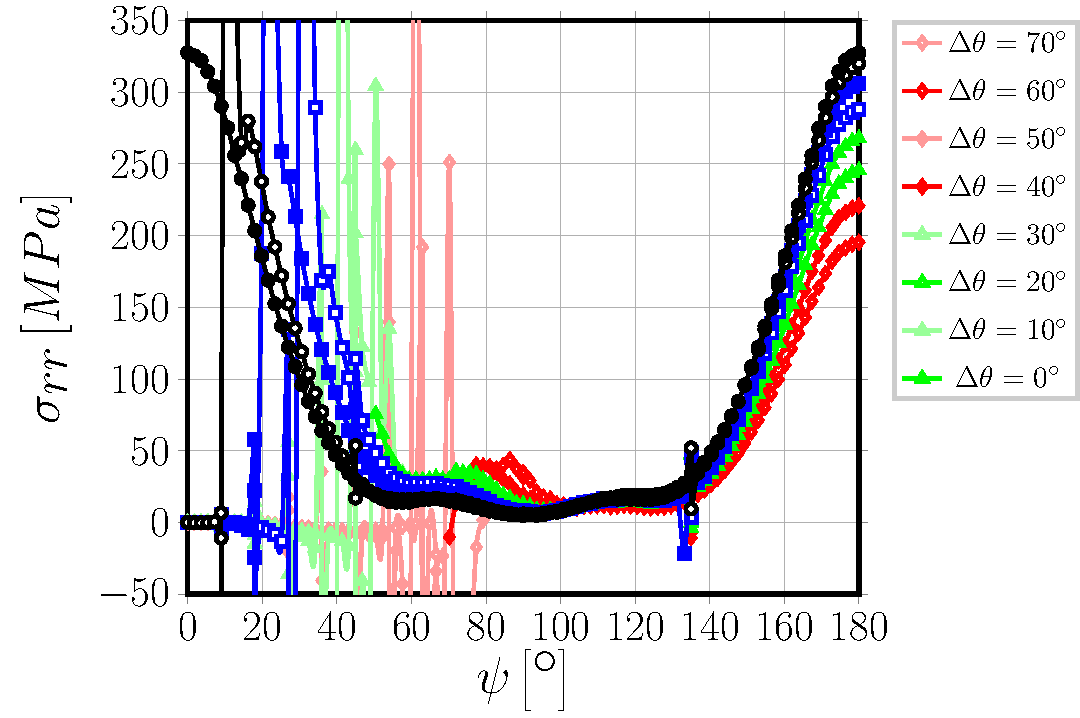
\includegraphics[width=\textwidth]{S5A0free-circum-sigmar.pdf}
\caption{$\sigma_{rr}$, $11\times 1-free$. $V_{f}=60\%$, $\varepsilon_{x}=1\%$.}\label{}
\end{figure}

\begin{figure}[!h]
\centering
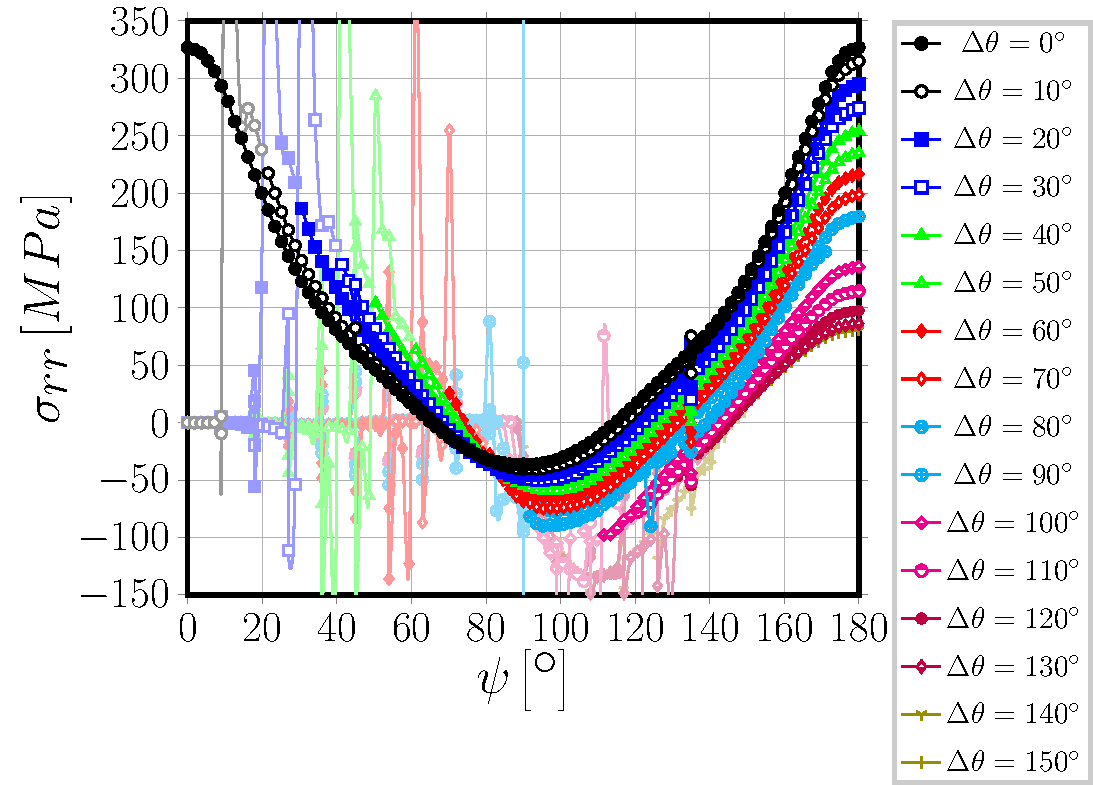
\includegraphics[width=\textwidth]{S5A0T1-circum-sigmar.pdf}
\caption{$\sigma_{rr}$, $11\times 1-1\cdot t_{90^{\circ}}$. $V_{f}=60\%$, $\varepsilon_{x}=1\%$.}\label{}
\end{figure}

\begin{figure}[!h]
\centering
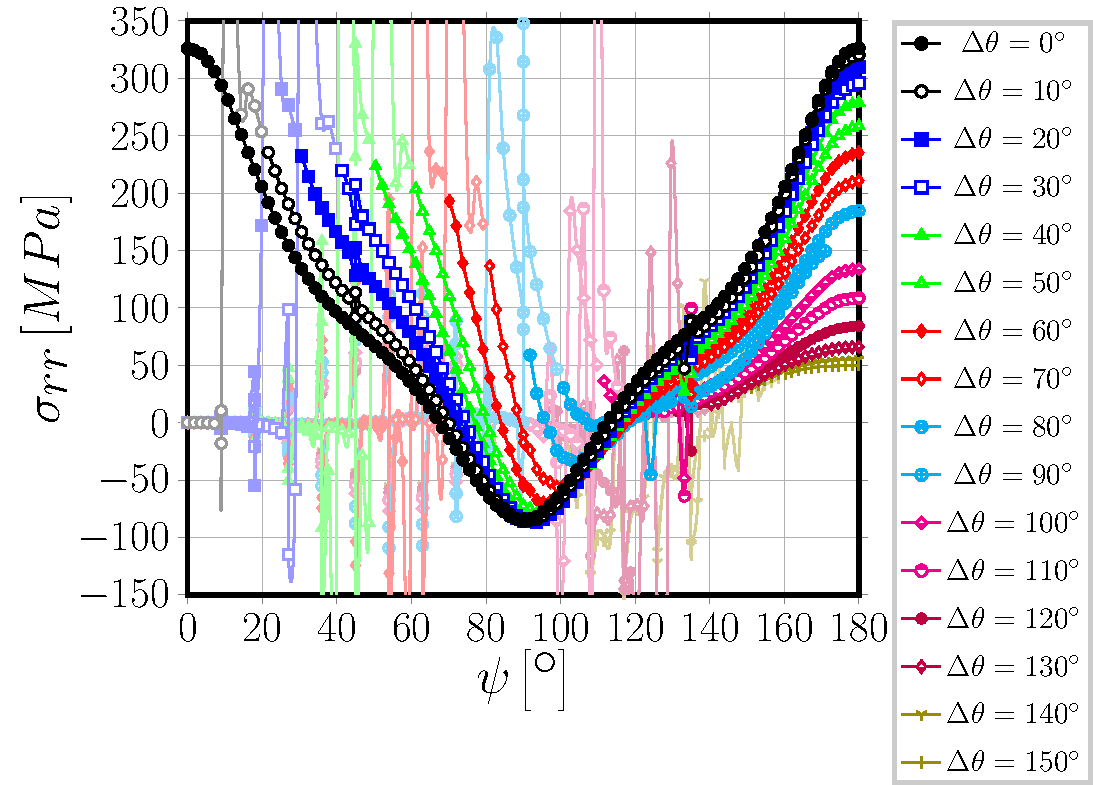
\includegraphics[width=\textwidth]{S5A0vk-circum-sigmar.pdf}
\caption{$\sigma_{rr}$, $11\times 1-symm$. $V_{f}=60\%$, $\varepsilon_{x}=1\%$.}\label{}
\end{figure}

\begin{figure}[!h]
\centering
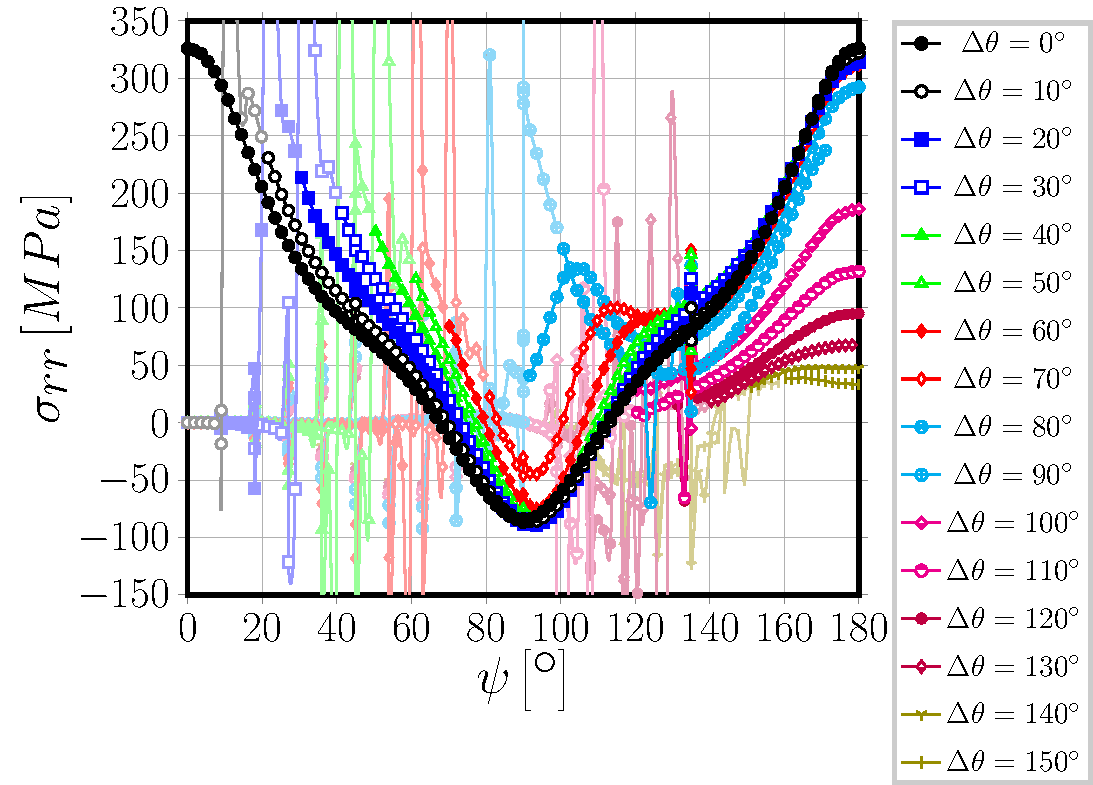
\includegraphics[width=\textwidth]{S5A0asymm-circum-sigmar.pdf}
\caption{$\sigma_{rr}$, $11\times 1-asymm$. $V_{f}=60\%$, $\varepsilon_{x}=1\%$.}\label{}
\end{figure}

\begin{figure}[!h]
\centering
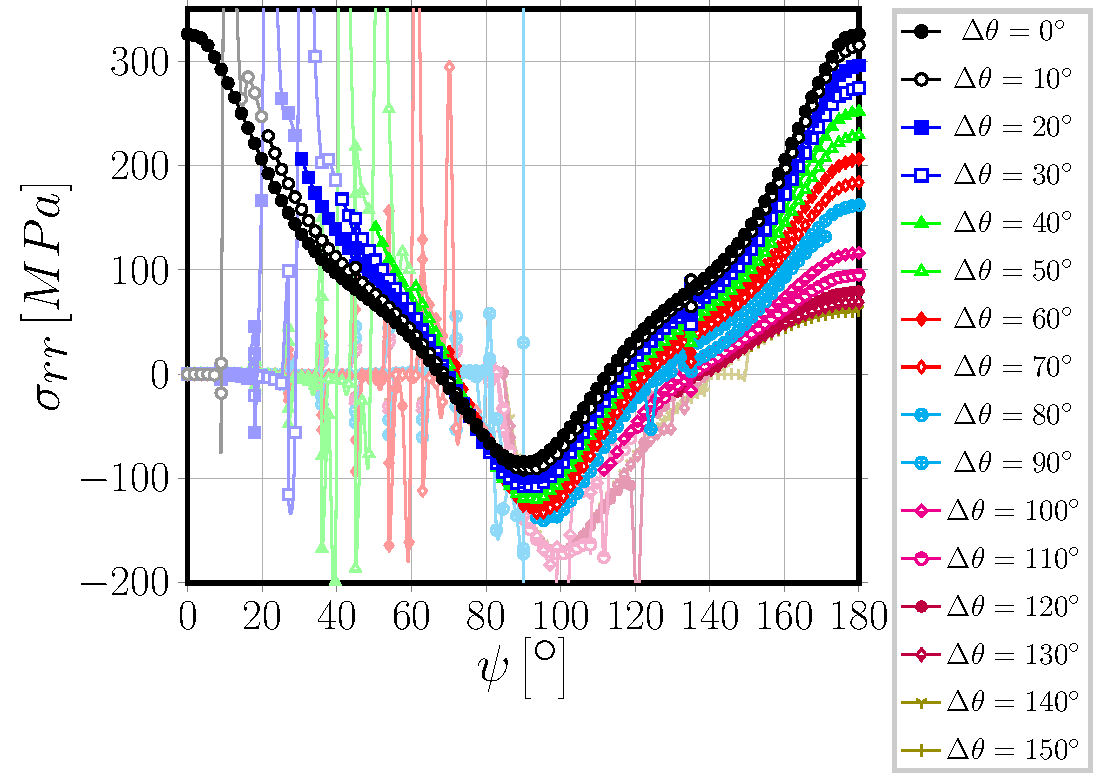
\includegraphics[width=\textwidth]{S5A1free-circum-sigmar.pdf}
\caption{$\sigma_{rr}$, $11\times 3-free$. $V_{f}=60\%$, $\varepsilon_{x}=1\%$.}\label{}
\end{figure}

\subsection{$\sigma_{\theta\theta}$}

\begin{figure}[!h]
\centering
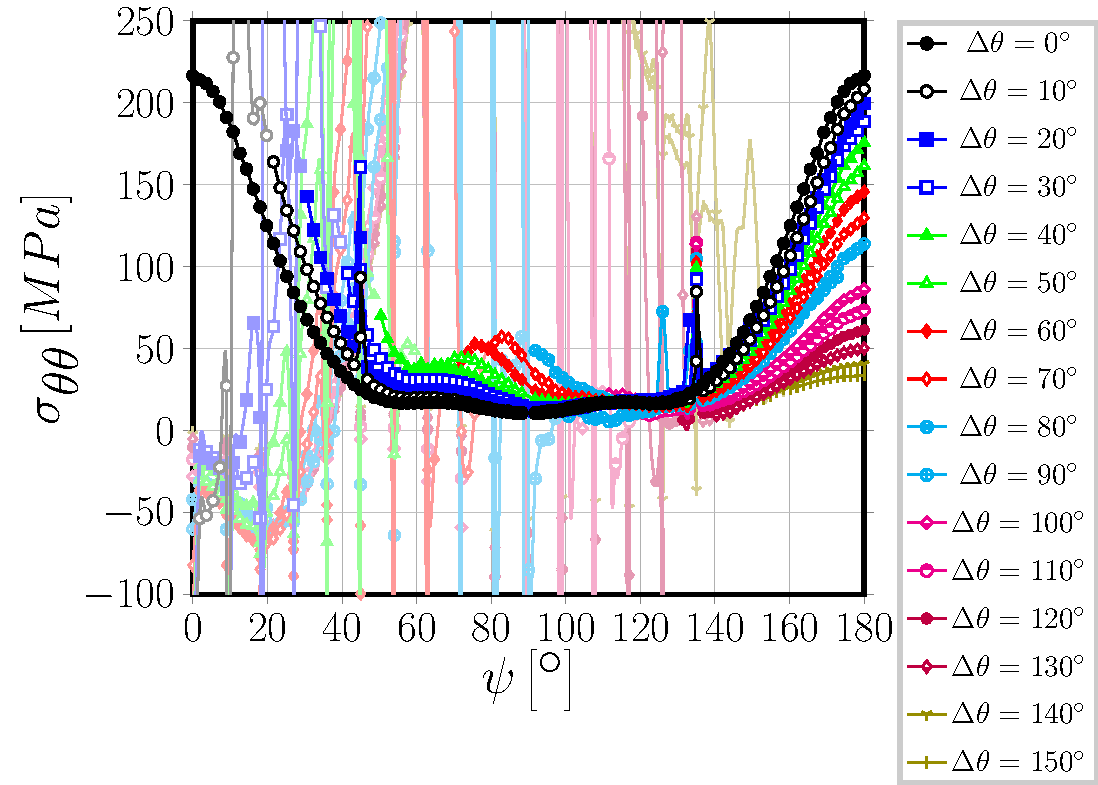
\includegraphics[width=\textwidth]{S5A0free-circum-sigmatt.pdf}
\caption{$\sigma_{\theta\theta}$, $11\times 1-free$. $V_{f}=60\%$, $\varepsilon_{x}=1\%$.}\label{}
\end{figure}

\begin{figure}[!h]
\centering
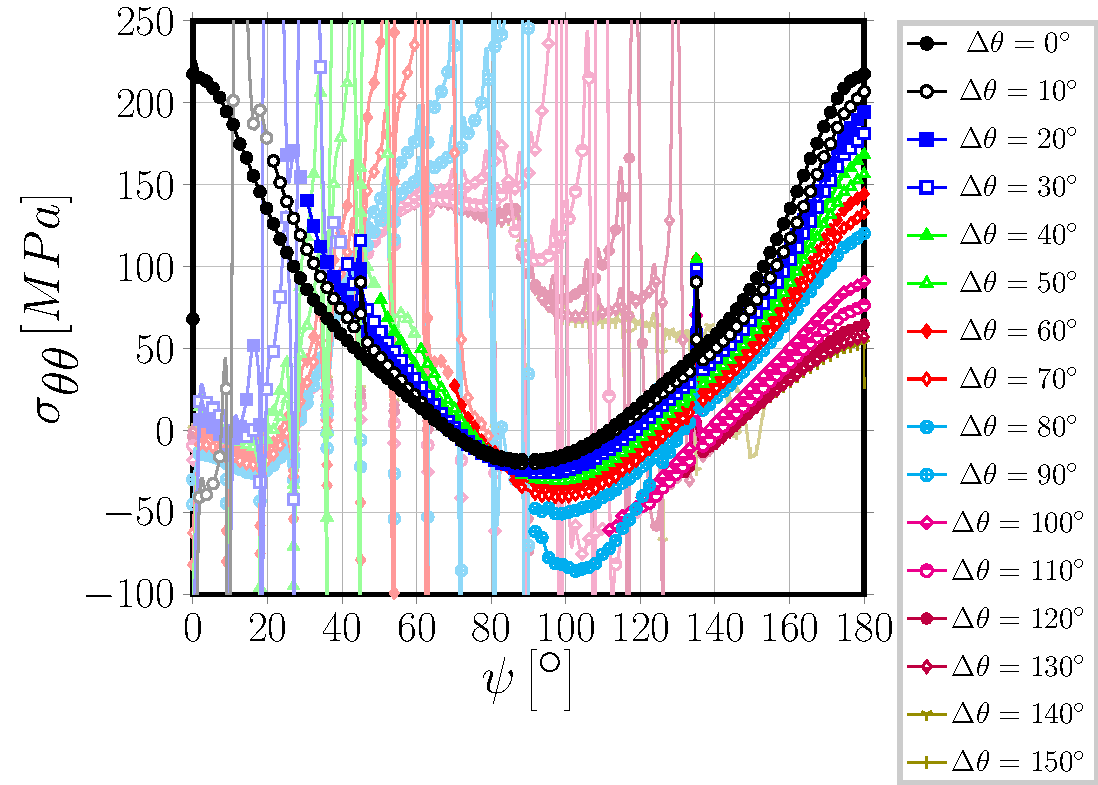
\includegraphics[width=\textwidth]{S5A0T1-circum-sigmatt.pdf}
\caption{$\sigma_{\theta\theta}$, $11\times 1-1\cdot t_{90^{\circ}}$. $V_{f}=60\%$, $\varepsilon_{x}=1\%$.}\label{}
\end{figure}

\begin{figure}[!h]
\centering
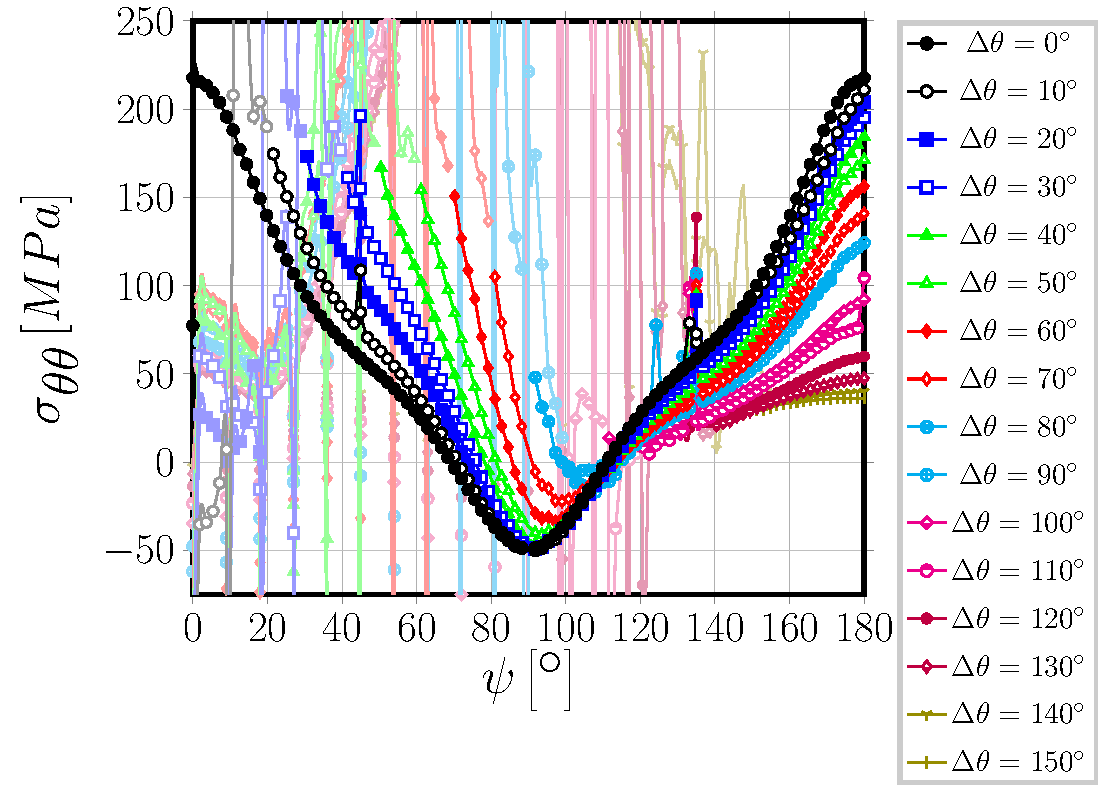
\includegraphics[width=\textwidth]{S5A0vk-circum-sigmatt.pdf}
\caption{$\sigma_{\theta\theta}$, $11\times 1-symm$. $V_{f}=60\%$, $\varepsilon_{x}=1\%$.}\label{}
\end{figure}

\begin{figure}[!h]
\centering
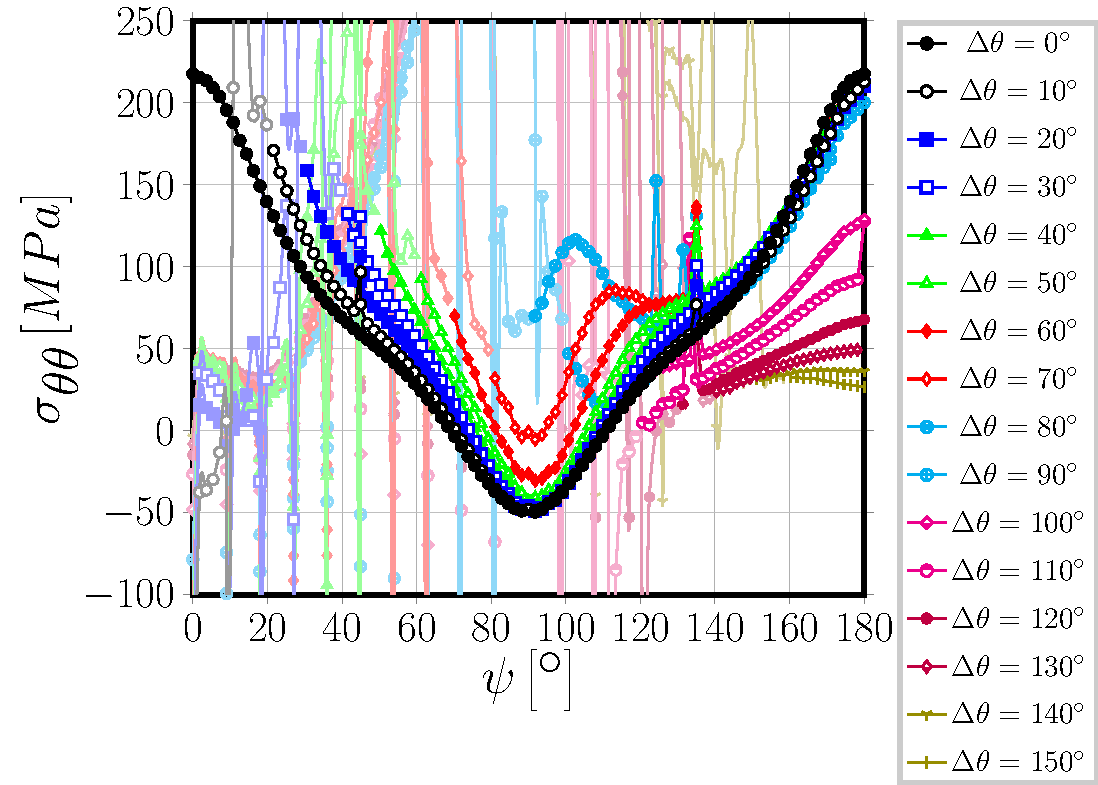
\includegraphics[width=\textwidth]{S5A0asymm-circum-sigmatt.pdf}
\caption{$\sigma_{\theta\theta}$, $11\times 1-asymm$. $V_{f}=60\%$, $\varepsilon_{x}=1\%$.}\label{}
\end{figure}

\subsection{$\tau_{r\theta}$}

\begin{figure}[!h]
\centering
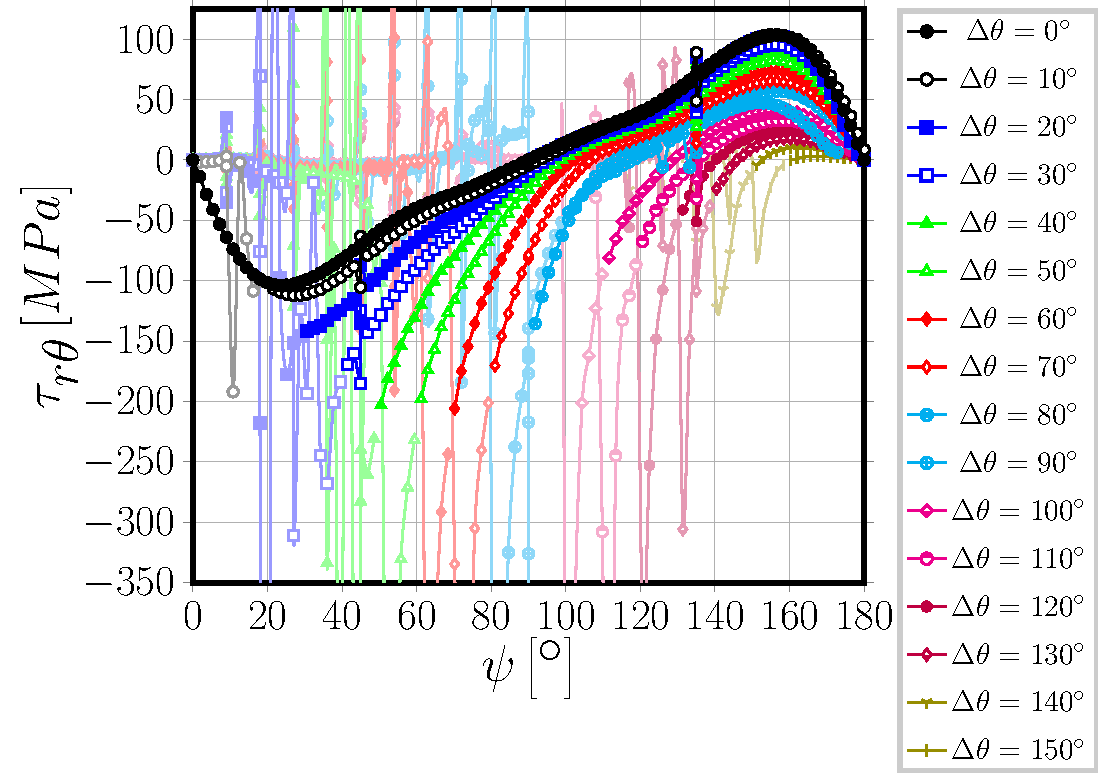
\includegraphics[width=\textwidth]{S5A0free-circum-taurt.pdf}
\caption{$\tau_{r\theta}$, $11\times 1-free$. $V_{f}=60\%$, $\varepsilon_{x}=1\%$.}\label{}
\end{figure}

\begin{figure}[!h]
\centering
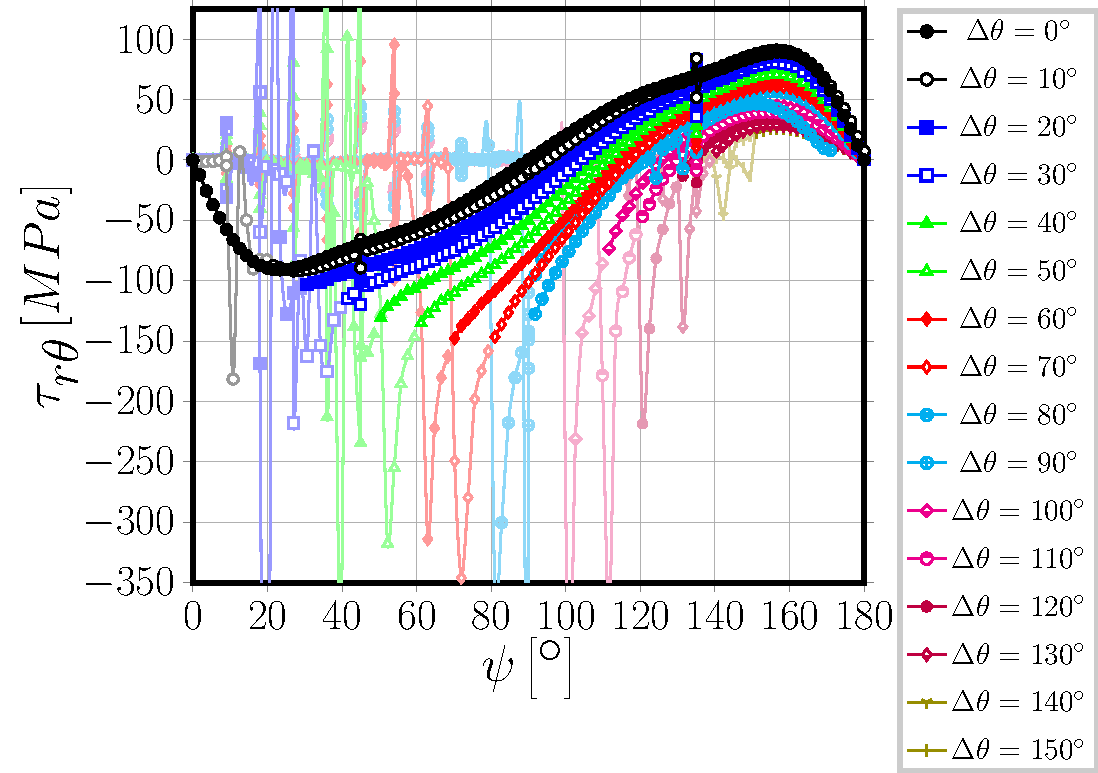
\includegraphics[width=\textwidth]{S5A0T1-circum-taurt.pdf}
\caption{$\tau_{r\theta}$, $11\times 1-1\cdot t_{90^{\circ}}$. $V_{f}=60\%$, $\varepsilon_{x}=1\%$.}\label{}
\end{figure}

\begin{figure}[!h]
\centering
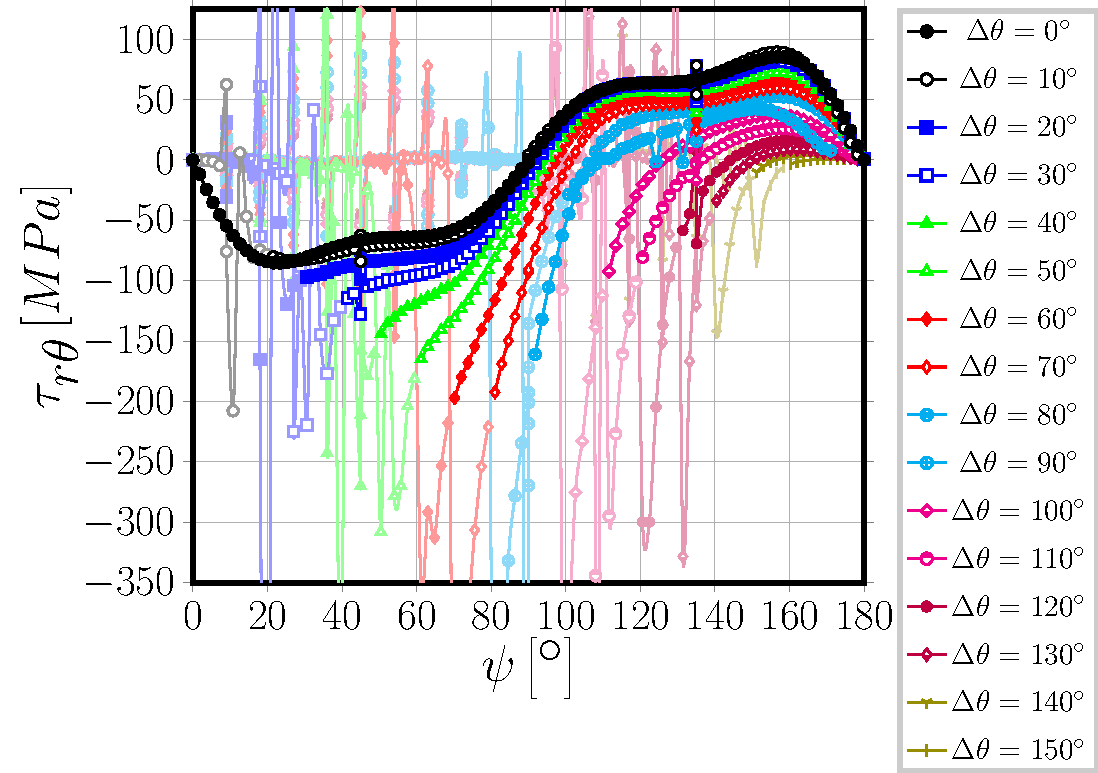
\includegraphics[width=\textwidth]{S5A0vk-circum-taurt.pdf}
\caption{$\tau_{r\theta}$, $11\times 1-symm$. $V_{f}=60\%$, $\varepsilon_{x}=1\%$.}\label{}
\end{figure}

\begin{figure}[!h]
\centering
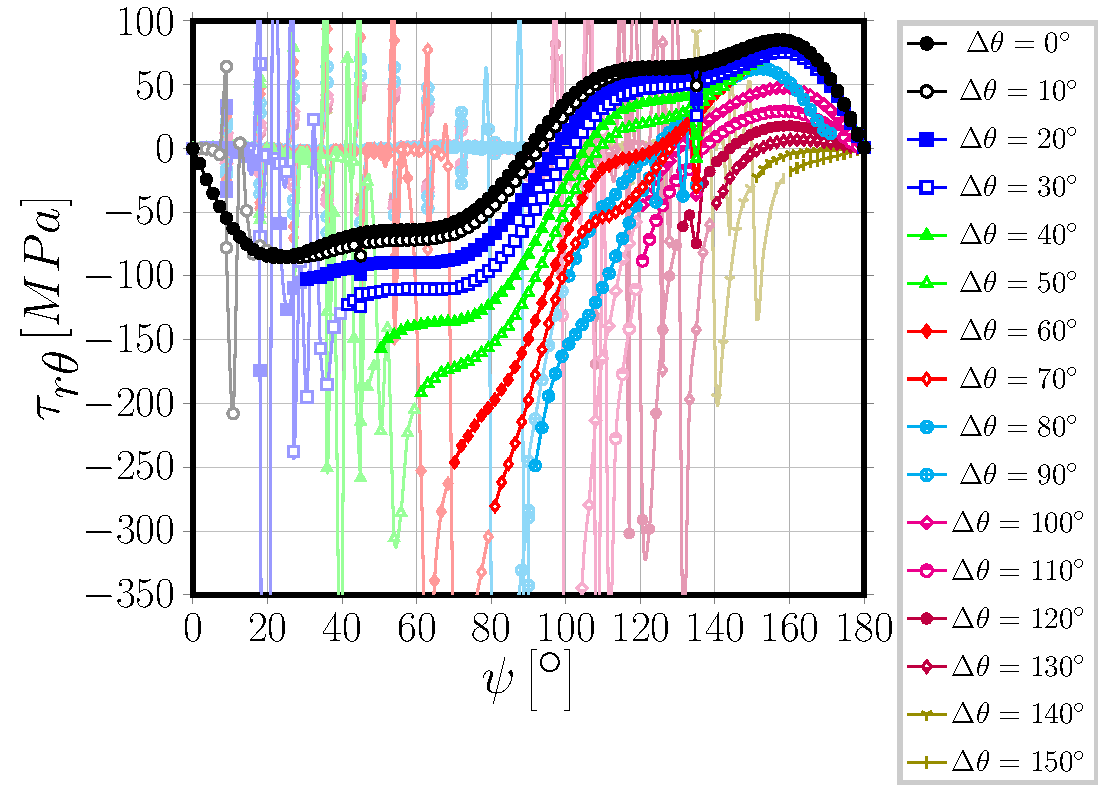
\includegraphics[width=\textwidth]{S5A0asymm-circum-taurt.pdf}
\caption{$\tau_{r\theta}$, $11\times 1-asymm$. $V_{f}=60\%$, $\varepsilon_{x}=1\%$.}\label{}
\end{figure}

\section{Conclusions}

\end{document}
